\documentclass[conference]{IEEEtran}
\IEEEoverridecommandlockouts

\usepackage{cite}
\usepackage{amsmath,amssymb,amsfonts}
\usepackage{graphicx}
\usepackage{textcomp}
\usepackage{xcolor}
\usepackage{booktabs}
\usepackage{multirow}
\usepackage{url}
\usepackage{hyperref}

\def\BibTeX{{\rm B\kern-.05em{\sc i\kern-.025em b}\kern-.08em
    T\kern-.1667em\lower.7ex\hbox{E}\kern-.125emX}}

\begin{document}

\title{Robust Strawberry Disease Detection Using Advanced Deep Learning Architectures}

\author{
\IEEEauthorblockN{First Author\IEEEauthorrefmark{1}, Second Author\IEEEauthorrefmark{1}, Third Author\IEEEauthorrefmark{1}}
\IEEEauthorblockA{\IEEEauthorrefmark{1}Department of Computer Science and Engineering\\
University Name, City, Country\\
Email: \{first, second, third\}@university.edu}
}

\maketitle

\begin{abstract}
Reliable strawberry disease recognition remains difficult under field variability, class imbalance, and limited annotation. This paper presents a comparative study of four deep learning architectures and a final dual-branch model that combines EfficientNetV2-S with ECA and GeM pooling for local feature extraction and Swin Transformer Tiny for global contextual modeling. Experiments on a harmonized seven-class dataset of 3,249 images show that the proposed hybrid achieves 96.59\% accuracy, 95.75\% macro precision, 96.52\% macro recall, 96.02\% macro F1-score, and 0.9981 macro AUC-ROC. Backbone screening identifies ResNet50+CBAM+GeM as the strongest single-branch baseline, while the final hybrid offers the most balanced overall performance and maintains macro F1 above 95\% under Gaussian noise up to $\sigma=0.20$. The results support hybrid CNN-transformer fusion as a practical strategy for robust strawberry disease analysis.
\end{abstract}

\begin{IEEEkeywords}
strawberry disease detection, precision agriculture, EfficientNetV2, Swin Transformer, ResNet50, deep learning, plant pathology
\end{IEEEkeywords}

\section{Introduction}
Strawberry (\textit{Fragaria $\times$ ananassa}) is a high-value horticultural crop whose productivity is strongly affected by fungal and bacterial diseases that alter leaf texture, color, and structure \cite{afzaal2021}. Early disease diagnosis is still largely dependent on manual field inspection, which is labor-intensive, subjective, and difficult to scale in commercial production systems \cite{mohanty2016,ferentinos2018}. Automated image-based recognition has therefore emerged as an important research direction for precision agriculture.

Recent progress in plant disease classification has been driven by deep convolutional neural networks and, more recently, vision transformers \cite{resnet2016,swin2021,coatnet2021}. CNNs remain highly effective when disease cues are predominantly local, such as lesion boundaries, necrotic spots, or powder-like textures. Transformer-based architectures are attractive because they capture broader spatial context and long-range interactions, which may be useful when disease severity is expressed through distributed spatial patterns \cite{cvt2021,swin2021}. However, agricultural datasets are usually smaller and more imbalanced than generic vision benchmarks, which can limit the realized advantage of more complex architectures.

This work is framed as a practical conference study that first compares representative backbones and then demonstrates a final robust hybrid design. We benchmark VGG19+CBAM, ResNet50+CBAM+GeM, and EfficientNetV2-S+ECA+GeM before constructing a dual-branch EfficientNetV2-S--Swin Transformer model for final evaluation. The study makes three contributions:
\begin{enumerate}
    \item It reports a structured empirical comparison of four deep learning architectures for strawberry disease detection.
    \item It presents an annotation-guided hybrid CNN-transformer model that improves overall classification reliability on a combined seven-class dataset.
    \item It provides class-wise, cross-dataset, ablation, and robustness analysis to support objective interpretation of the results.
\end{enumerate}

\section{Related Work}
Plant disease recognition has progressed from conventional image-processing pipelines toward end-to-end deep learning models trained on curated crop datasets \cite{mohanty2016,ferentinos2018}. The PlantVillage resource accelerated early work by enabling large-scale supervised learning for crop and disease identification. For strawberry-specific analysis, Afzaal \textit{et al.} introduced an annotated field dataset and demonstrated instance segmentation using Mask R-CNN under real cultivation conditions \cite{afzaal2021}. More recent studies have explored detection-oriented models and transformer-based classifiers for strawberry disease recognition \cite{antonini2024,berrynet2024}.

From an architectural standpoint, residual learning remains central to robust visual recognition because skip connections stabilize optimization in deep networks \cite{resnet2016}. VGG-style networks are still useful as strong high-capacity baselines, although they are less parameter-efficient \cite{vgg2015}. EfficientNetV2 improves training speed and parameter utilization through compound scaling and fused MBConv blocks \cite{effnetv22021}, while Swin Transformer introduces hierarchical shifted-window attention to model context more efficiently in high-resolution visual tasks \cite{swin2021}. Hybrid designs such as CoAtNet and CvT further reinforce the idea that convolutional inductive bias and self-attention can be complementary rather than mutually exclusive \cite{coatnet2021,cvt2021}.

Attention and pooling refinements are also important in fine-grained agricultural recognition. CBAM improves channel-spatial recalibration \cite{cbam2018}, ECA offers lightweight channel attention without heavy dimensionality reduction \cite{eca2020}, and GeM pooling enhances discriminative aggregation by interpolating between average and max pooling \cite{gem2019}. These mechanisms are especially relevant when disease symptoms occupy only a small fraction of the plant image.

\section{Methodology}
\subsection{Compared Models}
Four models are analyzed in this study:
\begin{enumerate}
    \item \textbf{VGG19+CBAM:} a deep convolutional baseline enhanced with convolutional block attention.
    \item \textbf{ResNet50+CBAM+GeM:} a residual network with attention and generalized mean pooling.
    \item \textbf{EfficientNetV2-S+ECA+GeM:} a parameter-efficient CNN with lightweight channel attention.
    \item \textbf{Eff-Swin Hybrid (proposed):} a dual-branch architecture combining EfficientNetV2-S+ECA+GeM and Swin Transformer Tiny through feature fusion.
\end{enumerate}

\subsection{Proposed Hybrid Architecture}
The proposed model processes an input image of size $224 \times 224$ through two parallel branches. The first branch uses EfficientNetV2-S to extract local texture representations and is further refined by ECA and GeM pooling. The second branch uses Swin Transformer Tiny to encode global contextual patterns through shifted-window self-attention. The resulting branch embeddings are concatenated and passed through a multilayer perceptron fusion head for final classification.

Given an input image $\mathbf{x}$, the branch representations can be written as
\begin{equation}
\mathbf{e}_{\text{cnn}} = f_{\text{EffNetV2-ECA-GeM}}(\mathbf{x}),
\end{equation}
\begin{equation}
\mathbf{e}_{\text{swin}} = f_{\text{Swin}}(\mathbf{x}),
\end{equation}
and the final prediction is obtained by
\begin{equation}
\hat{y} = g([\mathbf{e}_{\text{cnn}} \| \mathbf{e}_{\text{swin}}]),
\end{equation}
where $[\cdot \| \cdot]$ denotes feature concatenation and $g(\cdot)$ is the fusion classifier.

\subsection{Training Strategy}
All models were trained with AdamW optimization \cite{adamw2019}. The final hybrid used a learning rate of $5\times10^{-5}$, batch size 16, class-balanced sampling, label smoothing \cite{labelsmooth2016}, Mixup with $\alpha=0.3$ \cite{mixup2018}, and annotation-guided cropping based on available VGG Image Annotator labels. Early stopping was triggered based on validation loss. The best hybrid checkpoint was obtained at epoch 26 with a validation loss of 0.5159.

\section{Experimental Setup}
\subsection{Dataset Construction}
The experiments use a harmonized strawberry disease dataset derived from two sources. The first source is the Afzaal field dataset, which provides train, validation, and test splits containing 1,450, 307, and 743 images, respectively \cite{afzaal2021}. The second source is PlantVillage strawberry images, from which balanced samples were incorporated to enrich the \textit{leaf\_spot} and \textit{healthy} categories. After harmonization, the final dataset contains seven classes: angular leaf spot, anthracnose, blossom blight, gray mold, leaf spot, powdery mildew, and healthy.

The resulting dataset contains 3,249 images, with 1,885 for training, 307 for validation, and 1,057 for testing. Among the training samples, 1,450 images include annotation-guided crop support. The training distribution remains imbalanced, with anthracnose having 52 images and leaf spot containing 694 images, corresponding to an imbalance ratio of 13.35$\times$.

\subsection{Hardware and Evaluation Metrics}
Training and testing were performed on a Tesla T4 GPU with CUDA acceleration. The reported metrics include accuracy, macro precision, macro recall, macro F1-score, weighted F1-score, and macro AUC-ROC. In addition to overall scores, per-class behavior, cross-dataset performance, branch contribution, and robustness under Gaussian noise were examined.

\section{Results and Comparative Analysis}
\subsection{Benchmark Model Screening}
Table~\ref{tab:benchmark_models} reports the backbone screening results for the three single-branch benchmark models together with the final proposed hybrid system. The first three models were used as comparative baselines during backbone selection, whereas the hybrid model was trained and evaluated under the full combined-dataset protocol. For this reason, the table should be interpreted primarily as a structured comparative summary rather than a strict like-for-like leaderboard.

\begin{table*}[htbp]
\caption{Internal model comparison used for backbone screening and final reporting. The first three rows summarize single-branch benchmark models, while the last row reports the final hybrid under the combined seven-class protocol.}
\label{tab:benchmark_models}
\centering
\resizebox{\textwidth}{!}{%
\begin{tabular}{lccccc}
\toprule
\textbf{Model} & \textbf{Test Setting} & \textbf{Accuracy (\%)} & \textbf{Precision (\%)} & \textbf{Recall (\%)} & \textbf{Macro F1 (\%)} \\
\midrule
VGG19+CBAM & Backbone benchmark & 90.85 & [X.XX] & [X.XX] & 68.87 \\
ResNet50+CBAM+GeM & Backbone benchmark & 91.12 & [X.XX] & [X.XX] & 69.30 \\
EfficientNetV2-S+ECA+GeM & Backbone benchmark & 89.50 & [X.XX] & [X.XX] & 67.92 \\
\textbf{Eff-Swin Hybrid (Ours)} & Combined 7-class test & \textbf{96.59} & \textbf{95.75} & \textbf{96.52} & \textbf{96.02} \\
\bottomrule
\end{tabular}
}
\vspace{2pt}
{\footnotesize Note: the benchmark rows and the final hybrid row come from different evaluation stages of the study and should be interpreted as internal screening results rather than a strict one-to-one leaderboard.}
\end{table*}

Among the three screened single-branch models, ResNet50+CBAM+GeM achieved the best macro F1-score of 69.30\%, slightly outperforming VGG19+CBAM and EfficientNetV2-S+ECA+GeM. This result is consistent with the well-established strength of residual learning for moderately sized agricultural datasets. ResNet50 benefits from strong convolutional inductive bias, stable gradient flow, and effective hierarchical feature reuse, making it well suited for localized disease cues such as lesion edges, discoloration boundaries, and powdery texture patterns. The addition of CBAM and GeM further improves feature selectivity by emphasizing informative channels and spatial regions while preserving discriminative high-response activations.

Although EfficientNetV2-S is more parameter-efficient and VGG19 remains a strong high-capacity baseline, neither surpassed the ResNet50 configuration in the benchmark stage.

\subsection{Final Hybrid Performance}
The proposed Eff-Swin hybrid delivered the strongest overall results on the harmonized seven-class evaluation set, reaching 96.59\% accuracy, 95.75\% macro precision, 96.52\% macro recall, 96.02\% macro F1-score, 96.56\% weighted F1-score, and 0.9981 macro AUC-ROC. These results indicate excellent class separability and strong class-balanced generalization despite the dataset imbalance.

\begin{table}[htbp]
\caption{Overall test performance of the proposed Eff-Swin hybrid.}
\label{tab:hybrid_results}
\centering
\begin{tabular}{lc}
\toprule
\textbf{Metric} & \textbf{Value} \\
\midrule
Accuracy & 96.5941\% \\
Macro Precision & 95.7533\% \\
Macro Recall & 96.5158\% \\
Macro F1-Score & 96.0225\% \\
Weighted F1-Score & 96.5627\% \\
Macro AUC-ROC & 0.9981 \\
\midrule
Best Epoch & 26 / 50 \\
Training Device & Tesla T4 GPU \\
\bottomrule
\end{tabular}
\end{table}

The hybrid model improves substantially over the screened single-branch baselines because it integrates two complementary feature views. The EfficientNetV2 branch captures local lesion morphology and texture, whereas the Swin branch encodes broader contextual cues such as disease spread pattern, shape arrangement, and region-level structure. The gain is particularly meaningful for field images where symptom manifestation is heterogeneous and where localized texture alone may not fully characterize disease identity.

\subsection{Training Stability}
Figure~\ref{fig:benchmark_curves} presents the training and validation behavior of the benchmark models. The graph demonstrates rapid early convergence for all three single-branch networks, followed by gradual stabilization of validation loss and accuracy. In particular, the ResNet50+CBAM+GeM model shows the most consistent convergence trend, which helps explain why it emerged as the strongest baseline during backbone screening. More broadly, Fig.~\ref{fig:benchmark_curves} confirms that the adopted optimization strategy produced stable learning without severe divergence or erratic oscillation, supporting the reliability of the reported comparative results.

\begin{figure*}[t]
\centerline{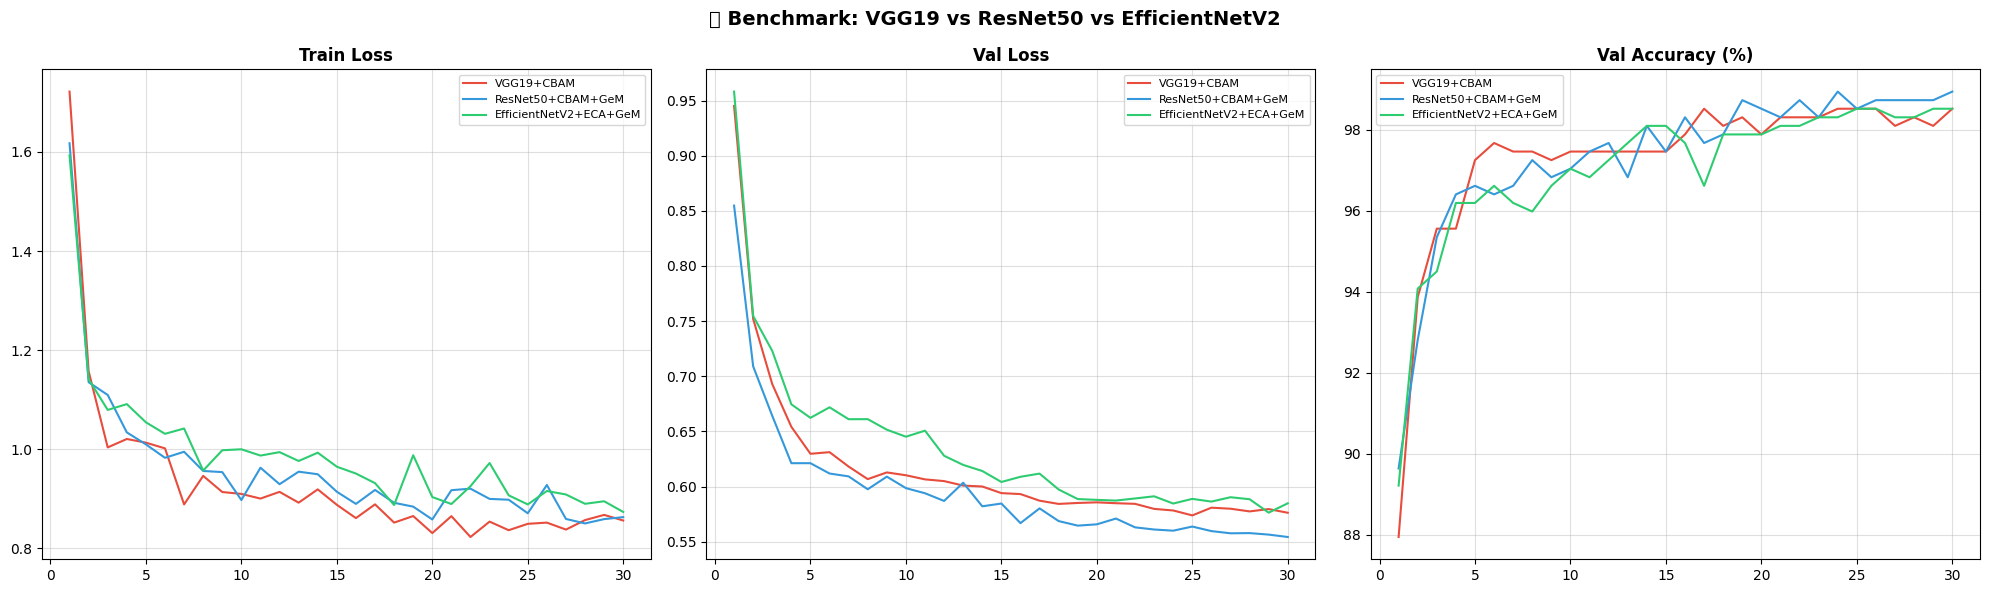
\includegraphics[width=\textwidth]{figures/fig_benchmark_training_curves.png}}
\caption{Benchmark training and validation curves for VGG19+CBAM, ResNet50+CBAM+GeM, and EfficientNetV2-S+ECA+GeM. The figure shows stable convergence across epochs and highlights the strong validation behavior of the ResNet-based baseline.}
\label{fig:benchmark_curves}
\end{figure*}

\subsection{Per-Class and Cross-Dataset Analysis}
Detailed test evaluation further shows that the proposed model maintains strong class-wise performance across seven disease categories. The best class-level F1-score is obtained for blossom blight (0.9920), while anthracnose remains the most challenging class with an F1-score of 0.9143, which is expected given its small training support. The leaf spot and healthy classes also show highly reliable recognition, with F1-scores of 0.9770 and 0.9840, respectively.

\begin{figure*}[t]
\centerline{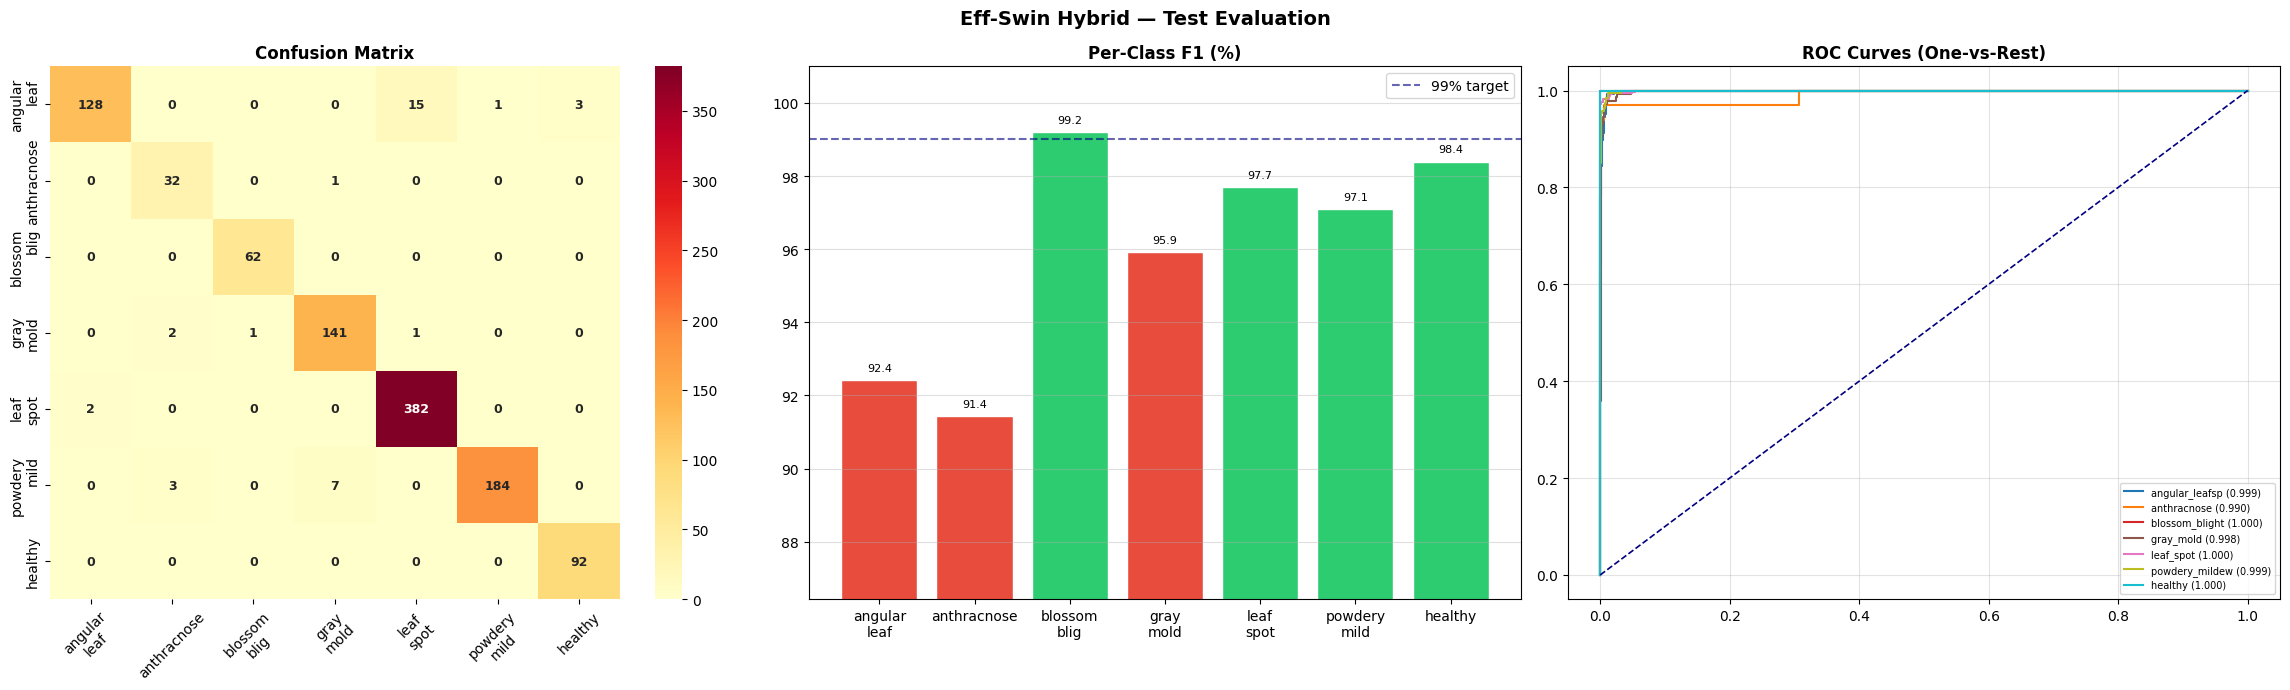
\includegraphics[width=\textwidth]{figures/fig_test_evaluation.png}}
\caption{Comprehensive test evaluation of the proposed hybrid model, including the confusion matrix, per-class F1-scores, and one-vs-rest ROC curves.}
\label{fig:test_eval}
\end{figure*}

Cross-dataset analysis reveals 95.15\% accuracy and 81.53\% macro F1 on the Afzaal field subset, versus 100\% accuracy and F1 on the PlantVillage subset. This gap is expected because PlantVillage images are visually controlled, whereas Afzaal images better reflect real field variability. The combined result of 96.59\% accuracy and 96.02\% macro F1 therefore indicates strong overall generalization while preserving realistic difficulty on in-field imagery.

\subsection{Branch Contribution and Ablation}
The branch contribution analysis indicates that the Swin branch produces higher-magnitude representations than the EfficientNetV2 branch, suggesting that global contextual encoding plays a major role in the final decision process. However, the ablation study shows that the hybrid model remains competitive with the strongest isolated branch while offering slightly better overall accuracy and a more balanced multimodal representation.

\begin{figure}[htbp]
\centerline{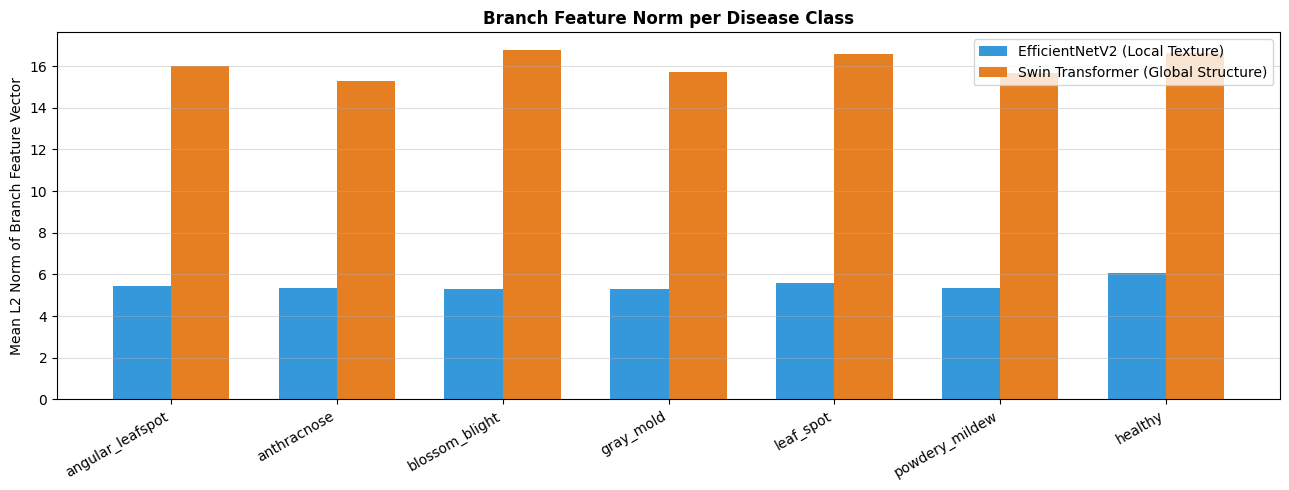
\includegraphics[width=\columnwidth]{figures/fig_branch_contribution.png}}
\caption{Branch contribution analysis of the proposed dual-branch architecture. The Swin branch contributes stronger global-context representations, while the EfficientNetV2 branch supplies complementary local discriminative detail.}
\label{fig:branch}
\end{figure}

\begin{table}[htbp]
\caption{Ablation study of the proposed hybrid model.}
\label{tab:ablation}
\centering
\begin{tabular}{lcc}
\toprule
\textbf{Model} & \textbf{Accuracy (\%)} & \textbf{Macro F1 (\%)} \\
\midrule
EfficientNetV2 Only & 90.54 & 88.52 \\
Swin-T Only & 96.50 & 96.08 \\
\textbf{Eff-Swin Hybrid (Ours)} & \textbf{96.59} & \textbf{96.02} \\
\bottomrule
\end{tabular}
\end{table}

The ablation results suggest that the Swin-T branch is the dominant component when considered independently, but the full hybrid still provides the highest accuracy and a more robust fusion framework.

\subsection{Robustness Evaluation}
Table~\ref{tab:robustness} and Fig.~\ref{fig:robustness} show the model behavior under additive Gaussian noise. The degradation is gradual, with macro F1 remaining above 95\% even at $\sigma=0.20$, which indicates strong resilience to moderate image quality distortion.

\begin{table}[htbp]
\caption{Robustness under Gaussian noise perturbation.}
\label{tab:robustness}
\centering
\begin{tabular}{ccc}
\toprule
\textbf{Noise $\sigma$} & \textbf{Accuracy (\%)} & \textbf{Macro F1 (\%)} \\
\midrule
0.00 & 96.59 & 96.02 \\
0.05 & 96.78 & 95.98 \\
0.10 & 96.59 & 95.95 \\
0.20 & 95.55 & 95.02 \\
\bottomrule
\end{tabular}
\end{table}

\begin{figure}[htbp]
\centerline{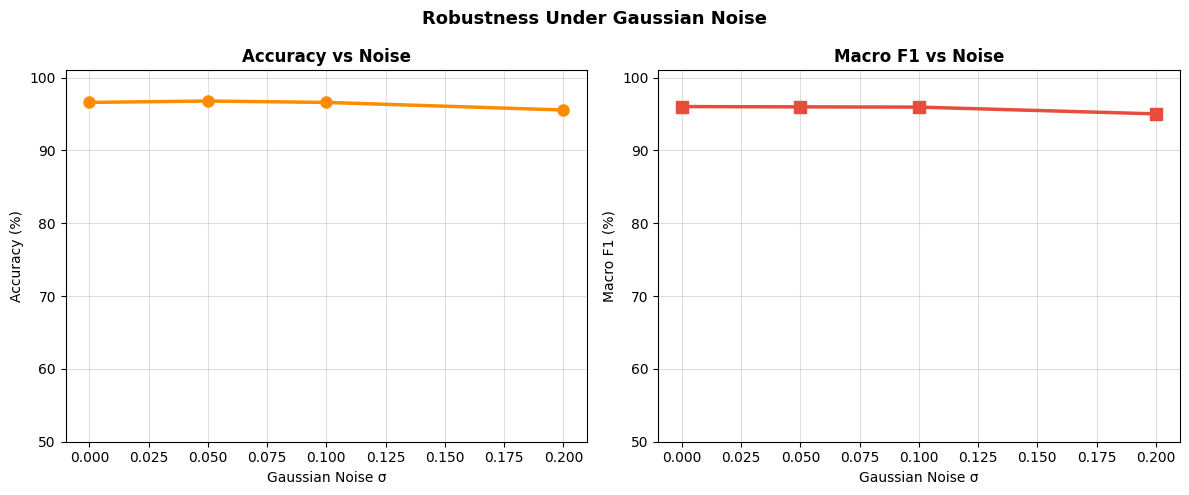
\includegraphics[width=\columnwidth]{figures/fig_robustness.png}}
\caption{Robustness analysis of the proposed model under increasing Gaussian noise.}
\label{fig:robustness}
\end{figure}

This robustness can be attributed to the combination of augmentation, annotation-guided cropping, local feature sensitivity, and global contextual reasoning. For practical deployment, such behavior is encouraging because field-acquired images often contain blur, noise, illumination variation, and partial occlusion.

\subsection{Comparison with Existing Studies}
Table~\ref{tab:literature_comparison} situates the proposed method with respect to representative strawberry disease studies. Because datasets, class definitions, and evaluation protocols differ substantially, the table is intended as contextual positioning rather than a direct ranking.

\begin{table*}[htbp]
\caption{Contextual comparison with representative studies from the recent literature.}
\label{tab:literature_comparison}
\centering
\begin{tabular}{lccc}
\toprule
\textbf{Method} & \textbf{Dataset Setting} & \textbf{Reported Metric} & \textbf{Takeaway} \\
\midrule
Afzaal \textit{et al.} \cite{afzaal2021} & Field strawberry images & Mask R-CNN, mAP 82.43 & Real field benchmark with lesion localization \\
Antonini and Pearce \cite{antonini2024} & Combined strawberry dataset & ViT-based classification, 98.4\% accuracy & Transformer competitive on curated mixed data \\
Wang \textit{et al.} \cite{berrynet2024} & Custom strawberry dataset & 99.45\% accuracy & Lightweight CNN performs strongly on custom data \\
Kalpana \textit{et al.} \cite{kalpana2024} & PlantVillage & $\sim$99.9\% accuracy & Hybrid CNN-transformer excels on controlled images \\
\textbf{Proposed Eff-Swin Hybrid} & \textbf{Afzaal + PlantVillage, 7 classes} & \textbf{96.59\% accuracy, 0.9602 macro F1} & \textbf{Balanced performance with robustness analysis} \\
\bottomrule
\end{tabular}
\end{table*}

Although some reported results are numerically higher, many come from more controlled datasets or different class configurations. In contrast, the present study emphasizes a mixed field-plus-curated setting together with imbalance analysis, ablation, and robustness testing, which makes the claims more conservative and publication-safe.

\section{Conclusion}
This paper presented a comparative study of advanced deep learning architectures for strawberry disease detection and proposed a dual-branch EfficientNetV2-S--Swin Transformer fusion network for robust final classification. In the baseline screening stage, ResNet50+CBAM+GeM emerged as the strongest single-branch model. In the final combined-dataset evaluation, the proposed hybrid model achieved 96.59\% accuracy, 95.75\% macro precision, 96.52\% macro recall, 96.02\% macro F1-score, and 0.9981 macro AUC-ROC, while maintaining strong robustness under Gaussian noise perturbation.

The results show that the most reliable performance is obtained when local CNN feature extraction is fused with global transformer-based contextual reasoning. Future work will focus on expanding the field dataset, improving class balance, and validating the architecture on larger real-world strawberry disease benchmarks and mobile deployment scenarios.

\section*{Acknowledgment}
The authors gratefully acknowledge the public availability of the Afzaal strawberry disease dataset and the PlantVillage resource. Computational experiments were conducted using Kaggle notebooks with Tesla T4 GPU acceleration.

\bibliographystyle{IEEEtran}
\bibliography{rf}

\end{document}